\documentclass[oneside,a4paper,11pt]{report}
%\usepackage[T1]{slovak}
\usepackage[utf8]{inputenc}
\usepackage{latexsym}
\usepackage{graphicx}
\usepackage{amsmath}
\usepackage{caption}
\usepackage{fancyhdr}
%\usepackage{picins}
\usepackage{times}
\usepackage{mathptmx}
\usepackage{url}
\usepackage{booktabs}
\usepackage{appendix}
\usepackage{rotating}
\usepackage{hyperref}
\pagestyle{fancy}
\fancyhead{}
\fancyhead[C]{\leftmark}
\renewcommand{\chaptermark}[1]{\markboth{\thechapter.\ #1}{}}


\usepackage[Sonny]{fncychap}
\makeatletter
 \ChNameVar{\small}
 \ChNumVar{\LARGE}
 \ChTitleVar{\LARGE\centering}
 \ChRuleWidth{0.05pt}
 \ChNameUpperCase

\usepackage{hyperref}
\newcommand\araa{ARA\&A}
\newcommand\aap{A\&A}
\newcommand\apj{ApJ}
\newcommand\apjs{ApJS}
\newcommand\mnras{MNRAS}
\usepackage{natbib}
% The astroads bibtex style formats the references according
% to the well-estabilished syntax in use in astronomy and
% creates a link if URLs are specified for a given record.

\bibliographystyle{astroads}


%\title{Štúdium premenných hviezd vo vysokoenergetickej části spektra}
\title{On stars in high energy }

\author{Matúš Kocka}



\begin{document}
%\begin{figure}
%\begin{center}
%
\includegraphics[width=6cm]{the-white-dwarf}
%\end{center}
%\end{figure}

\fancyhf{}
\newpage
\textit{"Per aspera ad astra..."}

\pagebreak
\tableofcontents

\addcontentsline{toc}{chapter}{\protect\numberline{}Introduction}
\chapter{Introduction to the stars in high energy }

Let your imagination soar. 
By sitting on the old rocker looking at the sky with couple of good old whiskey you can easily 
start thinking about the universe. You are looking at a heck of a different kinds of cosmic 
objects, but suddenly you see almost only the stars. Almost all the shiny dots on the sky are 
stars and these stars are only the closest ones. Yes, you can see few other 
galaxies by naked eye\footnote{M31 and M33 in extremely good conditions on northern hemisphere
and Magellanic clouds on southern one}, but none of the exotic cosmic objects you are imaging about. 
They are too faint to be observed easily, because they are not only far, far away, but they also usually shine 
on different wavelengths, not visible by human eye.

Think about distances in the universe. One of the most accurate explanation is that from: \cite{hitch:1}  
\textit{"Space," it says, "is big. Really big. You just won't believe how vastly, 
hugely, mindbogglingly big it is. I mean, you may think it's a long way down the road to the 
chemist's, but that's just peanuts to space..."} 

Consider this, sometimes you want to study processes in these extreme, very faint objects, 
but they are too faint and too far in the universe. You are looking for “laboratory” with similar
 processes, but located much closer to the observer. The X-ray binary stars can be this kind 
of laboratories.  

There is, of course, many interesting phenomena which could be studied in X-ray binaries or in non-binary X-ray stars. 
Several of them are mentioned in the motivation section. 

I am mentioning many interesting things in this work, but the main effort is taken to 
study post shock region in the Intermediate Polars (IPs).   


\section{Motivation}
We can easily find many reasons why to study stars in the high energy bands.  
We can consider the direct and the most common scientific applications like observations of 
the supernovae, black holes \& neutron stars in X-ray binaries. But for the education purposes 
I prefer several others, very nice examples closer to topic of this work.  

\begin{itemize}
 \item \textbf{Relativistic jet phenomena}: like it was proposed by \citet{mirabel:1} that universal 
mechanism should be at work in all the relativistic jet sources in the universe. Better understanding 
of sources including: microblazars, AGNs and gamma-ray burst will help to gain more comprehensive 
understanding of these phenomena. Microblazars can play role of “space laboratories”, where interesting
 processes last on different timescales as is the case with AGNs or GRBs.   

\begin{figure}[!hbt]
\centering
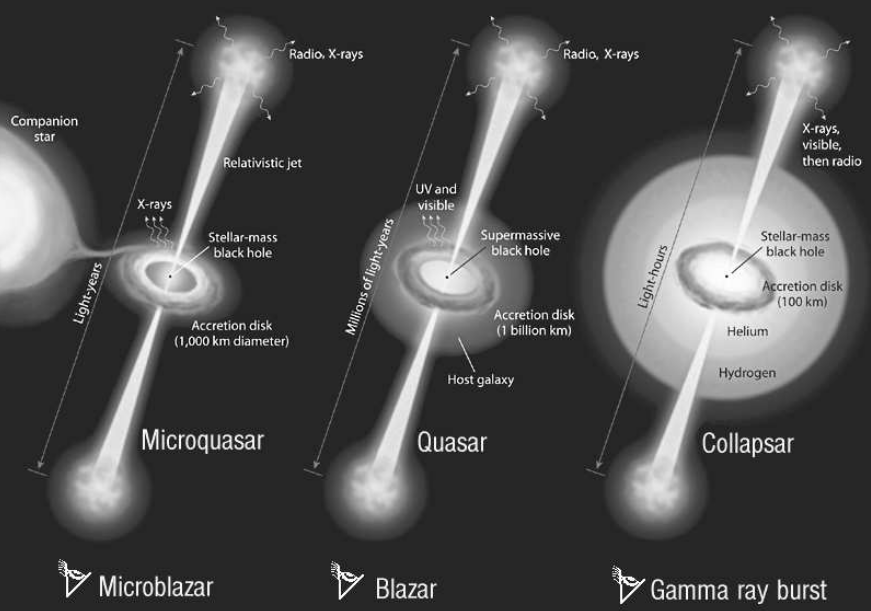
\includegraphics[totalheight=8.5cm]{microblazars}
\caption{NOT in scale diagram, showing curent ideas of micro-quasars, AGNs and gamma-ray
bursts as space objects driven by same, universal mechanism  \citet{mirabel:1}. }
\label{microblazar} 
\end{figure}

 \item \textbf{Galactic ridge X-ray emission (GRXE)}: various physical processes contribute to 
brightness of GRXE in different bands, but several studies in 3-20 keV provide evidence that diffuse 
X-ray radiation originates from huge number of stellar X-ray sources, mostly coronally active stars
 and white dwarf X-ray binaries. In particular for the energies over 20 keV to 200 keV is spectrum 
very similar to spectrum  of magnetic white dwarf binaries – e.g. Intermediate polars (IP) and polars (P).  
\citet{2007A&A...463..957K}
 
 \item \textbf{White dwarfs masses in Intermediate Polars (IP)}: as was proposed in \citet{1981ApJ...250..723R}, 
the temperature of the post shock region (PSR) depends on WD mass. Therefor the X-ray spectrum can be 
used for WD mass determination \citet{2005A&A...435..191S}. The WD mass estimations in cataclysmic stars 
is in general complicated. Usually the curve of radiation velocities can be used, but it is quit hard to constuct and
because of . 
Therefor X-ray spectrum method is very atractive for several reasons. This work is dedicated to this topic.  

\end{itemize}

\section{Aim of this work}
To cover the whole topic: ``stars in high energies'' is far behind capacity of such master thesis, because of that I decide 
to aim on cataclysmic variable stars (CVs), especialy to intermediate polars (IPs). 

As it will be mentioned in next sections closely, IPs are magnetized CVs where the compact, primary star 
is white dwarf with $B\sim 10^6 -10^7$ Gauss. The mass accretion is taking place from, mainly low-mass, non-degenerate star through Roche lobe.  
Accretion disk is in some distance from WD surface destroyed by strong magnetic field and 
accretion continuous through, so called, accretion curtain across magnetic force-field.

Falling material in some point creates stationary shock near the WD surface where the kinetic energy is converted 
through thermal bremsstrahlung to radiation. The temperature of such created plasma is typically more than 
10 keV with low density. The optically thin hard X-ray\footnote{In this case, hard X-rays means 10 - 120 keV region.} emission is taking place and heated gas creates 
post shock region (PSR) with temperature gradient. The hot gas then descends and cools by X-ray 
emission while it hits the WD surface.      

Because of relatively high temperature of PSR are IPs very good observed in hard X-rays band. 
IPs are only small fraction $\sim 15\%$ of all CVs, but they dominet in hard X-ray band over 10keV, ad most 
$\sim 80\%$ of detected CVs are IPs\citet{2009MNRAS.392..630L}. 

The temperature of PSR depends in first order only on WD mass, which is the most fundamental parameter of WDs.
This means, that if we are able to find temperature from fiting thermal bremsstrahlung model to spectrum of IP, 
we are also able to establis the WDs mass. 

An accrating WDs are very important for cosmology, because some of such objects probably casuse Type Ia supernovae, 
when the WD mass reaches Chandrasekhar limit. 

As is showed on figure~\ref{nylup1}, IP as NY Lup are well observed by INTEGRAL/IBIS detector which makes them 
iteresting space laboratories for WD basic parameters study. In same casesm, can by also accretion stream studied
if it is strong enough. 
    


\begin{figure}[!hbt]
\centering
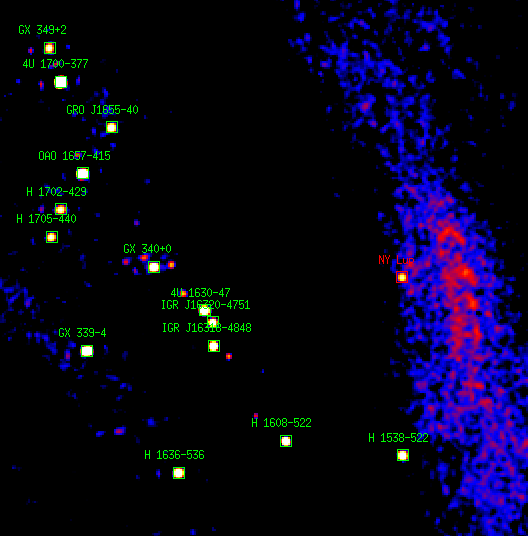
\includegraphics[totalheight=12cm]{plot/ds9_3}
\caption{1.2 Msec exposure of NY Lup region in 17-80 keV. The NY Lup is marked by red square. There are many others X-ray sources,
mostly HMXBs or LMXBs which is because of .}
\label{nylup1} 
\end{figure}



\section{Observations}
Cataclysmic Variable stars (CVs) have been, in fact, observed as early as ancient times. In historical 
records of  many civilizations we can find references for various astronomical events. Mostly they are 
about temporary objects: planets, Moon and Sun. However several are about comets and new stars. Rightly, 
these new stars are in many cases novae and supernovae. In China, the records date back to 1500 AD. 

Many records are saved from medieval time, for example positions of \textit{Nova Vulpecula 1670} and 
\textit{Nova Cygni 1600} (now knows as P Cygni) in Hevelius maps. 

With progress of astronomical photography in late 19th century started era of continuous observations
and with  development of first photo-multipliers in the mid-1940s CVs were begun attractive 
targets because of their big variability in different time scales. 

It is suitable to mention, that AAVSO has light curve of SS Cyg from 1896 up to date. 
\subsection{Optical and IR observations}
The very first visual observation was follows by photographic photometry and then spectroscopy, 
follows by photo-multiplier photometry since mid-1940s. The binary nature of all the CVs was confirm. 
The flickering was discovered and was assumed that it is somehow connected to stars duplicity Walker (1957),
\citet{warner:1}.

Statistical studies by Luyten and Hughes in mid-1960th showed, that novae remnants have $M_V \approx 4$ and 
dwarf novae at quisence have $M_V \approx 7.5$. They conculde that the hot primary star in CVs must by WD or 
 hot subdwarf \citet{warner:1}.   

The most important contribution of optical astronomy to this work is the discovery of large and 
variable circular polarization in several CVs. This helped to identified magnetic CVs, 
which were later divided to two categories, polars and intermediate polars.

There are more important discoveries in optical and IR bands in CVs subject. In case of interest the 
 \citet{warner:1} is proper book. 
   
   
\subsection{X-ray observations}
The very first CV detected in X-rays was the EX Hya observed by Uhuru X-ray space mission. 
Uhuru  works in 2.0 – 6.0 keV and in spite of its poor sensitivity the well-known 4U catalogue
 was created \citet{1978ApJS...38..357F} from its observations.

The NASA`s HEAO\footnote{High Energy Astronomy Observatory, The HEAO 2 was also known as 
The Einstein Observatory} program follows with three space missions. As the X-ray detectors 
technology evolves, the number of detected CVs grown linearly. \mbox{EXOSAT} provided long and 
uninterrupted data of many CVs during his operation from May 1983 until April 1986. 
Similar results were obtained from Soviet mission \mbox{Kvant 1} and Japan's Ginga.
The high hopes were entered into ROSAT which provides all-sky survey in the
 0.1 – 2.0 keV but expected huge number of new CVs was not discovered. 

The situation slightly changes with RXTE\footnote{Rossi X-ray Timing Explorer} which after 
years on orbit provides good data for several articles about WD masses \citet{2005A&A...435..191S}. 
The data from RXTE are used in new articles even $\sim15$ years after its launch \citet{2011A&A...526A..77B}.
 
Several others missions were launched in last ten years period. Few of them caried several 
detectors where one was sensitive in X-rays, like SUZAKU/XIS and Swift/XRT. But for the X-ray 
astronomy was been the year of 1999 the most important ever. The two major big observatories 
was launched on the Earth's orbit. The Chandra X-ray Observatory onboard STS-93 space shuttle 
Columbia on July and the XMM-Newton launched onboard ESA's Ariane 5 rocket.

   That was the beginning of the X-ray astronomy's golden era. During last decade the combination of 
Chandra and XMM provides enormous data archives which will be useful for astronomers for another 
decades. 

Sadly, there will not be such big observatory in X-rays for several decades. Only bigger space 
mission is Japan's ASTRO-H with several X-ray and gamma ray detectors on-board to cover broad 
high energy bands. The future of big ESA \& NASA space mission Athena (formerly: Constellation-X, 
XEUS, IXO)  is questionable because of budget cuts in both space agencies. 

Fortunately, there are several data archives with open data for anybody 
interested. This is big challenge mainly for young astronomers, who are 
not in any big space mission program but want to do science. In this case, 
they don't need any special hardware, even modern laptops are powerful enough.     



    
\subsection{Gamma ray observations}
In last millennium several space mission observed few CVs in bands from tents of keV to TeV.\footnote{The most 
studied CV from this era is AE Aqr (Meintjes 1990; Bowden et al. 1991)}
The biggest breakthrough came with ESA's INTEGRAL space mission which was able with its sensitivity 
and large field of view observed many CVs. Mostly intermediate polars. Only $\sim 2\%$ 
of all CVs are actually magnetic ones, but those ones are only visible in gamma rays.
INTEGRAL/IBIS was been used to determine white dwarf masses by \citet{2009MNRAS.392..630L}.

Two others space missions have on-board detectors similar to INTEGRAL/IBIS with their sensitivity 
and coverage: the NASA's Swift/BAT and Japan's Suzaku/XRT. Both are widely used to study white dwarf 
masses in IPs \citet{2009A&A...496..121B}, \citet{2010A&A...520A..25Y}.    



\chapter{White Dwarfs}


\chapter{Cataclysmic variable stars}
\section{Non magnetic cataclysmic variables} 
\section{Magnetic cataclysmic variables}
\subsection{Polars}
\subsection{Intermediate polars}
\section{Galactic population ofcataclysmic variables }
\section{Others important creatures}
\section{GXRE}



\chapter{Masses of white dwarfs in intermediate polars}
\section{Breaking radiation}
\subsection{Bremsstrahlung}
\begin{equation}
 a_{\parallel} = \dot{v}_x = -\frac{eE_x}{m_e}\frac{\gamma {Z_e}^2 vt}{4\pi \varepsilon_0 m_e \left [ b^2 + \left ( \gamma vt \right )^2  \right ]^{2/3}} 
\end{equation}

\subsection{Thermal bremsstrahlung}



\section{Synchrotron radiation}
\section{Post shock region}
\section{WD mass estimations methods}

\chapter{Data analysis}

\section{INTEGRAL}

\begin{figure}[!hbt]
\centering
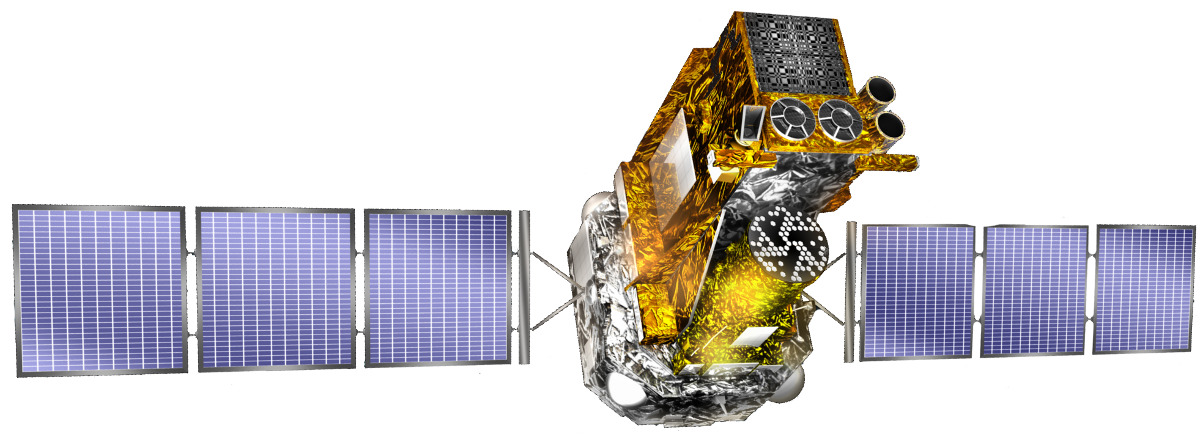
\includegraphics[totalheight=4cm]{integral}
\caption{INTEGRAL}
\label{microblazar} 
\end{figure}


\section{XMM-Newton}

\begin{figure}[!hbt]
\centering
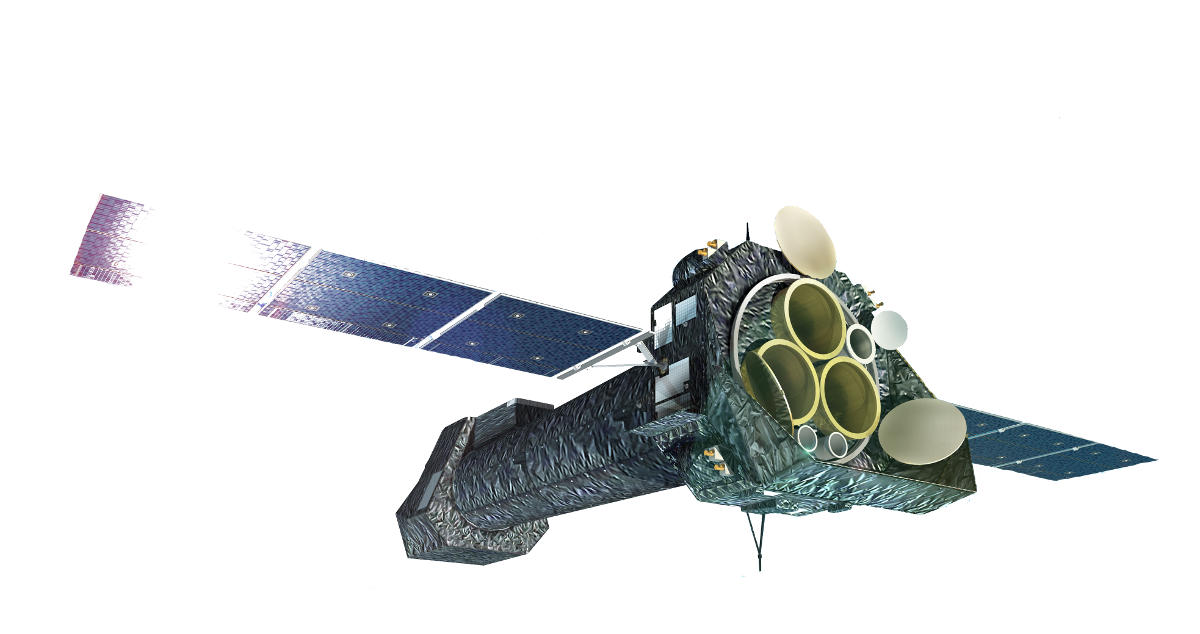
\includegraphics[totalheight=6cm]{XMM}
\caption{XMM-Newton }
\label{microblazar} 
\end{figure}


\section{Results}
\section{Discussion}
\chapter{Conclusions}



%\section{Hmotnosť bieleho trpaslík}
%\subsection{Pomocou kontinua}
%\subsection{Pomocou K železných čiar}
%\chapter{Spracovanie dát}
%\section{INTEGRAL}
%\section{XMM-Newton}
%\chapter{Určenie hmotností vybraných IP}



%\chapter{Intermedialne polary}   

\nocite{2004bhwd.book.....S}
\nocite{2009A&A...496..121B}
\nocite{accpower:1}
\nocite{2005A&A...435..191S}
\nocite{2008A&A...489.1121R}
\nocite{2010A&A...520A..25Y}
\nocite{warner:1}
\nocite{2006A&A...450..117S}
\nocite{rybicki:1}
\nocite{1973PThPh..49.1184A_aizu}
\nocite{astrop_techniques_5th}
\nocite{xray_hanbook}
\bibliography{koci}
\addcontentsline{toc}{chapter}{\hspace*{6mm}Bibliography}



\clearpage

\appendix
\section*{Appendix}
\addcontentsline{toc}{chapter}{\hspace*{6mm}Apendix}
this will be the appendix
%\pagebreak



\begin{sidewaystable}
\begin{center}
 

\caption{Estimated WD masses from previous reports ...}
\begin{tabular}{llllllll}
\hline
\hline
%\multicolumn{2}{c}{Item} \\
System & Suzaku & Swift & RXTE & RXTE & Ginga & ASCA& This work  \\
       & XIS+HXD & BAT& PCA+HEXTE & PCA & LAC & SIS & XMM \& Integral                     \\
       & $M_{WD}$ &$M_{WD}$ &$M_{WD} $&$M_{WD}$ &$M_{WD}$ &$M_{WD}$ &$M_{WD}$ \\
\hline
 FO Aqr      &         &        &          &     &      &         &           \\
 XY Ari      &         &        &          &     &      &         &           \\
 MU Cam      &         &        &          &     &      &         &           \\
 BG CMi&         &        &          &     &      &         &           \\
 V709 Cas&         &        &          &     &      &         &           \\
 TV Col&         &        &          &     &      &         &           \\
 TX Col&         &        &          &     &      &         &           \\
 YY Dra&         &        &          &     &      &         &           \\
 PQ Gem&         &        &          &     &      &         &           \\
 EX Hya&         &        &          &     &      &         &           \\
 NY Lup&         &        &          &     &      &         &           \\
 V2400 Oph&         &        &          &     &      &         &           \\
 AO Psc&         &        &          &     &      &         &           \\
 V1223 Sgr&         &        &          &     &      &         &           \\
 RX J2133&         &        &          &     &      &         &           \\
 IGR J17303&         &        &          &     &      &         &           \\

\hline
\end{tabular}

\end{center}
\end{sidewaystable}
%\thispagestyle{empty}
%\LaTeX{}
\end{document}


